\documentclass[12pt,twoside,openright]{memoir}
\stockaiv

\usepackage{tikz}

\begin{document}

\part{Introduction to Chart}                   % Print a "part" heading
\chapter{Stars and Signs}                % Print a "chapter" heading

The Houses are divisions in space (or in time) of the energy field of the earth, such that there is a twelve-fold division, paralleling the twelve-fold division of the Zodiac (the signs). Just like the signs, the houses also reveal an unfolding pattern of growth and development, from the First House to the Twelfth House.\\*

The 1st, 5th and 9th houses are FIRE houses involved with identity.\\*

The 2nd, 6th and 10th houses are EARTH houses concerned with the material plane. \\*

The 3rd, 7th and 11th houses are AIR houses involved with communication and relationship. \\*

The 4th, 8th, and 12th houses are WATER houses concerned with the depths of the soul or psyche. \\*

It is said that the planets are specific energies, modulated by the energy of their sign, which play themselves out in the department of your life represented by their particular house position. \\*


\section {Ascendant}
Indicates the Cusp of the First House. The Ascendant, or Rising Sign, is the mask shown to others, the way we present ourselves. This sign, along with the sign of the Sun and the sign of the Moon, is an important component of your personality. The sign on the Ascendant often describes one's physical appearance. Those with Leo Rising, for example, are likely to possess a mane of flowing hair. Planets in conjunction with the Ascendant also affect personality and appearance, in accordance with the qualities of the particular planet. The Ascendant represents your persona, or how you appear to others, how others sense you, in your true interaction with the world. In esoteric tradition, the Ascendant represents your true or soul-level personality.\\*

\section {First House}
The First House symbolizes the acting self, the personality as it appears to others, and the unfolding of one's individual destiny. Its beginning point is the Rising sign degree, one of the most significant points in the birthchart. Planets in the First House affect your personality strongly. Their characteristics are a keynote of your personality as you express yourself to others.

\section {Second House}
The Second House symbolizes what the self has to work with materially: possessions, money, and physical resources. This house also represents your desires and values. Planets in the Second House operate in the field of material needs and also indicate what you value most highly.

\section {Third House}
The Third House symbolizes thinking and communication, also traditionally brothers and sisters, writings, and short journeys. Your early environment is also represented by this house, as well as your powers of analysis and discrimination. Planets in this house indicate how you communicate and operate mentally.

\section {Nadir or IC}
Indicates the cusp of the Fourth House. As the base of operations of the personality this house is quite important, because without a place to stand emotionally, the personality cannot function.

\section {Fourth House}
The Fourth House represents the home environment, family life, and the father, or perhaps the same sex parent. Planets in the Fourth House reflect your family orientation, an ability to dig into the past in order to discover the roots of your being, and how your father (or perhaps your mother) was experienced by you.

\section {Fifth House}
The Fifth House represents creativity and self-expression, also offspring, and is also associated with romance and affection. Following the base of operations represented by the fourth, the fifth house represents the arena in which your personal energies can be released into the world. Any area which is stamped by your personality, including the display of affection or any creative endeavors such as your artistic expression, is therefore represented by planets in the Fifth House or the sign on the Fifth House cusp.

\section {Sixth House}
The Sixth House represents issues of sickness and health, and service to others, including conditions of daily life, or work. This house also relates to discipleship and mastery, and the overcoming of obstacles in producing the fruit of one's achievements. Planets in this house can manifest as challenges to your well-being, or as indications of a profession of service to others.

\section {Descendant}
Indicates the cusp of the Seventh House. The sign on the Descendant often indicates the type of marriage partner you will seek.

\section {Seventh House}
The Seventh House represents marriage and partnerships of all kinds, and issues with relating to other people. As the opposite to the First House of personality, the Seventh House describes how you fit into the world of others. Planets in this house often indicate the type of marriage partner you will seek.

\section {Eighth House}
The Eighth House symbolizes issues of death and rebirth, sexuality, and transformation. As this house follows the house of relationship, it refers to the fruits of relationship, and these include the power to change based on new understanding made possible when one is no longer acting solely as an individual. Planets in this house are difficult to interpret, but may refer to how sexuality is manifested or to lessons you need to learn in order to grow and change.

\section {Ninth House}
The Ninth House represents intuition and the study of religion philosophy, and higher learning. In addition, it represents travel to other countries, and legal matters. This house is interpreted similarly to the ninth sign of Sagittarius, and represents the expansion of horizons, mental, physical and spiritual. Planets in this house may symbolize your philosophical pursuits, or possibilities for travel.

\section {Midheaven or MC}
The Midheaven or MC (Medium Coeli) usually, but not always, indicates the %tenth house% cusp. Symbolically, the Midheaven represents your individuality, the outward expression of your energies. It can also be referred to as ego identity, and has a strong connection with public life and career, as symbolized by the %tenth house%. The Midheaven also represents your aspirations and ideals. Together with the %ascendant%, it represents personality in interaction with the world. Natal planets in conjunction with the Midheaven are considered "elevated" and are emphasized in the chart.

\section {Tenth House}
The Tenth House symbolizes the public life, authority, career issues, and also represents the mother, or perhaps the opposite-sex parent. As standing opposite the Fourth House, the Tenth House represents how the foundation of the personality is made manifest and concrete in the world. The birth chart is often divided into four seven-year periods, one per quadrant, cycling each twenty-eight years of life, and the Tenth House is reached at age 21, the age of legal adulthood. Planets in the Tenth House will indicate what the energies and challenges are for your career, and also how your mother (or perhaps father) was experienced.

\section {Eleventh House}
The Eleventh House symbolizes goals and objectives, also friendships and membership in groups or associations. The work in society represented by the tenth house is released through the individual in the activities associated with the eleventh house. Planets in this house indicate how visions for the future and also group associations and friendships will operate in your life.

\section {Twelfth House}
The Twelfth House refers to the unconscious and to things beyond the physical plane. It is traditionally associated with confinement and self-undoing, and has been called the house of karma. Planets in this house indicate functions that are hidden from your conscious personality, and are expressed in terms of psychic faculty or self-sacrifice. \\*\\*

\begin{figure}
\center
\caption{Sample Chart}
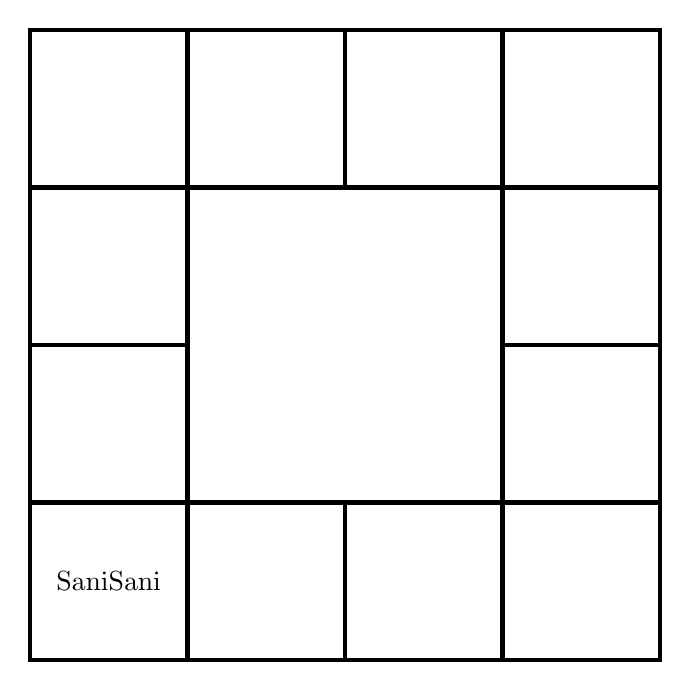
\begin{tikzpicture}
\draw[black,ultra thick] (0,0) rectangle (8,8);

\draw[black,ultra thick] (0,0) rectangle (2,2) node[pos=.5]  {Sani \\ Sani};
\draw[black,ultra thick] (2,0) rectangle (4,2);
\draw[black,ultra thick] (4,0) rectangle (6,2);
\draw[black,ultra thick] (6,0) rectangle (8,2);

\draw[black,ultra thick] (8,2) rectangle (6,4);
\draw[black,ultra thick] (8,4) rectangle (6,6);

\draw[black,ultra thick] (8,6) rectangle (6,8);
\draw[black,ultra thick] (6,6) rectangle (4,8);
\draw[black,ultra thick] (4,6) rectangle (2,8);
\draw[black,ultra thick] (2,6) rectangle (0,8);

\draw[black,ultra thick] (0,6) rectangle (2,4);
\draw[black,ultra thick] (0,4) rectangle (2,2);

\end{tikzpicture}
\end{figure}

\end{document}